\subsection{$I$ Multinomial Distributions}
The contingency Table for this design looks the same
\begin{figure}[H]
	\centering
	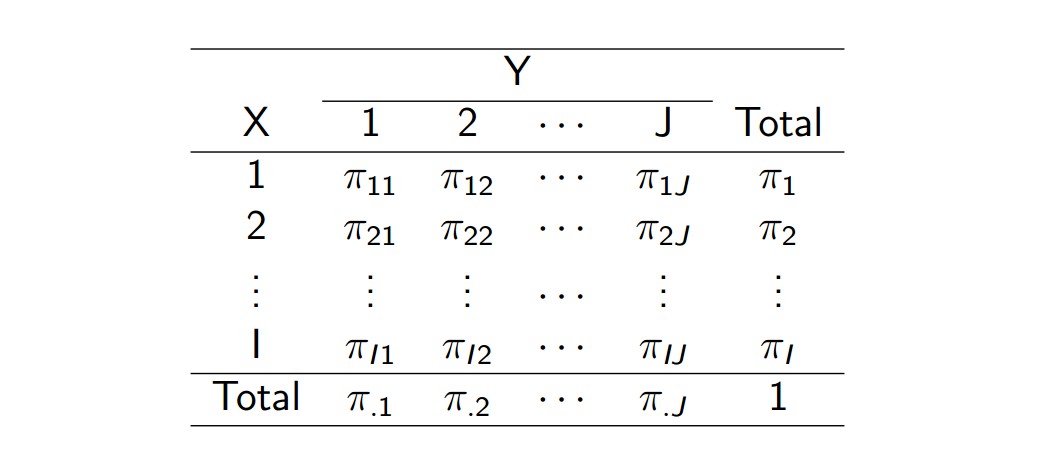
\includegraphics[width=0.7\linewidth]{fig/screenshot002}
	\caption{Example of Contingency Table}
	\label{fig:screenshot003}
\end{figure}

We have a separate $J$-category multinomial distribution in each of the $I$ groups. Define $\pi_{j|i} = \P(Y = j| X = i)$ as the probability of observing response category $j$ given that a unit is from group $i$.
\[\sum_{j= 1}^{J} \pi_{j|i} = 1, ~\text{for each } i = 1, \cdots, I.\]

The probability of observing a sequence $z_{i1}, \cdots, z_{iJ}$ from group $i$ is
\[\P(n_{i1} = z_{i1}, \cdots, n_{iJ} = z_{iJ}|n_i = \frac{n!}{\prod_{j=1}^{J} n_{ij}!} \prod_{j=1}^{J} \pi_{j|i}^{n_{ij}}\]

The full model for the contingency table is the Product Multinomial Model
\[\prod_{i=1}^{I} \frac{n!}{\prod_{j=1}^{J} n_{ij}!} \prod_{j=1}^{J} \pi_{j|i}^{n_{ij}} \]

\subsection{Independence}
Independence of $X$ and $Y$ in the context of a product multinomial
model means that the conditional probabilities for each $Y$ are equal
across the rows of the table.

For each $j = 1, \cdots J$, we have
\begin{itemize}
	\item $\P(Y = j| X = 1) = \cdots = \P(Y = j| X = I) = \P(Y = j)$.
	\item $\pi_{j|1} = \cdots = \pi_{j|I} = \pi_{.j}$
	\item $\hat{\pi}_{j|i} = \frac{n_{ij}}{n_i} = \frac{n_{ij}}{n} / \frac{n_i}{n} = \frac{\hat{pi}_{ij}}{\hat{\pi}_i}$.
\end{itemize}

Note that this condition is mathematically equivalent to
independence as defined for the one multinomial model.

\begin{proof}
	Because $X$ is not random in the product multinomial model, we
	define $\pi_i$ to be the fixed proportion of the total sample that is
	taken from group $i$.
	
	Then $\pi_{j|i} = \frac{\pi_{ij}}{\pi_i} = \pi_{.j}$
together imply that $\pi_{ij} = \pi_i \pi_{.j}$
\end{proof}

\subsection{Summary}
\begin{itemize}
	\item Parameter estimates from the one and product multinomial
	models are the same.
	\item The definitions of independence in the two models are
	equivalent.
	\item The two models lead to exactly the same conditional
	distributions for $Y$ given $X = i$.
	\item As a consequence, analyses conducted based on each model
	generally yield the same results.
	\item Therefore, when developing tests for independence and other
	analyses on contingency tables, we assume whichever model for
	the table is most convenient.
\end{itemize}